%%%%%%%%%%%%%%%%%
%	Paquetes	%
%%%%%%%%%%%%%%%%%

\documentclass[osajnl,twocolumn,showpacs,superscriptaddress,10pt]{revtex4-1}
%
\usepackage{dcolumn}% Align table columns on decimal point
\usepackage{bm}% bold math
%
%Paquete de Idioma
\usepackage[spanish]{babel}
%
%Codificación Alfabeto
\usepackage[utf8]{inputenc}
%
%Codificación de Fuente
\usepackage[T1]{fontenc}
%
%Índice
\usepackage{makeidx}
%
%Gráficos
\usepackage{graphicx}
\usepackage{subfig}
%\usepackage{xcolor} 
%
%Matemática
\usepackage{amsmath}
\usepackage{amsfonts}
\usepackage{amssymb}
%\usepackage{amstext} 
%
%Estilo de Página Numeración superior
%\pagestyle{headings}
%
%Hiperlinks \href{url}{text}
\usepackage[pdftex]{hyperref}
%
%Graficos y tablas
\usepackage{multirow}
%\usepackage{multicol}
\usepackage{float}
\usepackage{booktabs}
%
\decimalpoint
%\bibliographystyle{IEEEtran}
%\bibliography{IEEEabrv,mybibfile}
%Para tachar dimencionales
\usepackage{cancel}
%
%

%<<<<<<<<< Comando valores absolutos |x| >>>>>
\providecommand{\abs}[1]{\lvert#1\rvert}
%<<<<<<<<< Comando para la normal ||x|| >>>>>
\providecommand{\norm}[1]{\lVert#1\rVert}

%<<<<<<<<< para saltos de página usar  \clearpage >>>>>
%<<<<<<<<< para saltos entre líneas usar \vspace{2cm}>>>>>
%<<<<<<<<< para espaciado horizontal \hspace{1cm}>>>>>
%<<<<<<<<< para colocar url o referencias a url usar \url{http://www.latex-project.org/} o  \href{http://www.latex-project.org/}{latex project}>>>>>>>



%Paquete para configurar medidas de las tablas
\usepackage{tabularx}
%Forma del comando
%\begin{tabular}{|m{0.22\linewidth}|m{0.22\linewidth}|}


%<<<<<<<<< Para configurar \begin{enumerate}[A)]  en donde está la letra "A" escogemos como queremos enumerar, ejemplo \begin{enumerate}[i)]>>>>>>>>>>>>>>
\usepackage{enumerate}

%<<<<<<<<< Cambiar columnas >>>>>
%Se aconseja colocar el documento a una columna y luego cambiarle con forme se vaya utilizando. comandos:
%\begin{multicols}{2}
	%contenido
%\end{multicols}
%\usepackage{multicol} %Paquete cambiar columnas



\begin{document}


%%%%%%%%%%%%%%%%%%%%%%%%%%%%%
%	Autores y filiaciónes	%
%%%%%%%%%%%%%%%%%%%%%%%%%%%%%

%Titulo
\title{Práctica 1: Circuito de diente de sierra con SCR}
\thanks{Laboratorios de electrónica 4}

\author{Héctor Fernando Carrera Soto, 201700923}\email{e-mail: 3505043180101@ingenieria.usac.edu.gt}
\affiliation{Facultad de Ingeniería, Escuela de ingeniería mecánica eléctrica, Universidad de San Carlos, Edificio T1, Ciudad Universitaria, Zona 12, Guatemala.
}%
%\author{Nombre, Apellido, carne}\email{e-mail: correo2@dominio2}
%\affiliation{Facultad de Ingeniería, Departamento de Física, Universidad de San Carlos, Edificio T1, Ciudad Universitaria, Zona 12, Guatemala.
%}%
%\author{Nombre, Apellido, carne}\email{e-mail: correo3@dominio3}
%\affiliation{Facultad de Ingeniería, Departamento de Física, Universidad de San Carlos, Edificio T1, Ciudad Universitaria, Zona 12, Guatemala.
%}%

%\collaboration{MUSO Collaboration}%\noaffiliation

%\date{\today}%


%%%%%%%%%%%%%%%%%
%	Resumen		%
%%%%%%%%%%%%%%%%%

\begin{abstract}

    Se realizó un circuito generado de señal, diente de sierra. Se comprendió y entendió el uso del componente SCR, así como la identificación de cada uno de sus puertos. Se utilizó el teorema de Thevening para comprender el funcionamiento del circuito propuesto.

\end{abstract}

%%%%%%%%%%%%%%%%%
%	Encabezado	%
%%%%%%%%%%%%%%%%%


\maketitle{}

%%%%%%%%%%%%%%%%%
%	Objetivos	%
%%%%%%%%%%%%%%%%%

\section{Objetivos}

    %Es necesario indicar de manera el propósito del trabajo. Definir los objetivos de la práctica permite la formulación de una o varias hipótesis. Los objetivos se pueden clasificar en objetivos generales y específicos.
    

\begin{itemize}
    \item[*] Mostrar utilizando un SCR, cómo se puede crear una salida en diente de sierra, en el cual el período es determinado por la constante de tiempo.
    
    \item[*] Mostrar que en un circuito cuya alimentación es una fuente de valores medianos o altos, es muy importante hacer previamente un cálculo teórico de las corrientes que circulan a su través para evitar daños a los componentes una vez puesta en operación.
\end{itemize}
 
%%%%%%%%%%%%%%%%%%%%%
%	Marco teórico	%
%%%%%%%%%%%%%%%%%%%%%
 
\section{Marco Teórico}

    %Su contenido debe tener una exposición lógica y ordenada de los temas, así como evitar la excesiva extensión y el resumen extremo de la presentación de la teoría. Es importante que la teoría expuesta no sea una "transcripción bibliográfica" de temas que tengan alguna relación con el problema, sino que fundamente científicamente el trabajo.\\
    
\subsection{SCR}

El rectificador controlado de silicio es un tipo de tiristor formado por cuatro capas de material semiconductor con estructura PNPN o bien NPNP. El nombre proviene de la unión de Tiratrón (tyratron) y Transistor. Un SCR posee tres conexiones: ánodo, cátodo y gate (puerta). La puerta es la encargada de controlar el paso de corriente entre el ánodo y el cátodo. Funciona básicamente como un diodo rectificador controlado, permitiendo circular la corriente en un solo sentido. Mientras no se aplique ninguna tensión en la puerta del SCR no se inicia la conducción y en el instante en que se aplique dicha tensión, el tiristor comienza a conducir. Trabajando en corriente alterna el SCR se desexcita en cada alternancia o semiciclo. Trabajando en corriente continua, se necesita un circuito de bloqueo forzado, o bien interrumpir el circuito.\\

\begin{figure}[H]
\centering
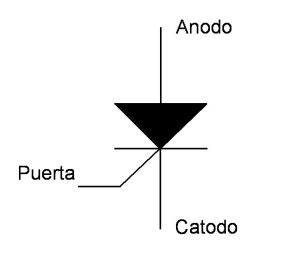
\includegraphics[scale=0.35]{Tiristor.png}
\caption{Esquema de un teristor.}
\end{figure}

\subsection{Teorema de Thevening}

El Teorema de Thevenin es uno de los enunciados básicos de la teoría de circuitos, a través del cual es posible
calcular y simplificar un circuito eléctrico complejo entre dos puntos o terminales A y B, obteniendo un circuito equivalente más simple. El enunciado se desglosa de la siguiente manera: Si el circuito original posee muchas resistencias, y se desea calcular intensidad, tensión o potencia de alguna de estas, o que se ubique entre los puntos A y B de un circuito grande, se puede simplificar el proceso a través del teorema de Thevenin. Se establece que es posible construir un circuito equivalente más pequeño, comprendido por una resistencia y una fuente de tensión dispuestos en serie. Los valores asignados a cada uno de estos se conoce como resistencia de Thevenin y tensión de Thevenin, que serán equivalentes al valor de la resistencia entre A y B, conocida como resistencia de carga.

\begin{figure}[H]
\centering
\includegraphics[width = \columnwidth]{Análisis.png}
\caption{Esquema de un circuito de Thevening.}
\end{figure}


%%%%%%%%%%%%%%%%%%%%%%%%%%%%%
%	Diseño experimental		%
%%%%%%%%%%%%%%%%%%%%%%%%%%%%%

\section{Diseño Experimental}

    %Hace una descripción del método o técnica utilizada para medir y/o calcular las magnitudes físicas en estudio, y si es del caso, del aparato de medición. Hay que recordar que el "método" es el procedimiento o dirección que conducirá a la solución del problema planteado. Se recomienda redactar una breve introducción para explicar el enfoque metodológico seleccionado.\\

Para calcular la frecuencia sabemos que:\\

\begin{equation}
f_{\textup{frec}} = \dfrac{1}{T}
\label{frec}
\end{equation}

Donde T, es el periodo de la señal, la cual se encuentran en el apartado de anexos.

\begin{equation}
V_{1} = \dfrac{V_{o}}{R_{3}/(R_{2} + R_{3})}
\label{V_in}
\end{equation}

Para deducir el voltaje máximo que puede alcanza el capacitor.

\begin{equation}
V_{out} = \dfrac{R_{2} + R_{3}}{R_{1}} * V_{c}
\label{V_0}
\end{equation}

Para la ecuaón

%%%%%%%%%%%%%%%%%
%	Mateiales	%
%%%%%%%%%%%%%%%%%

\subsection{Materiales}

\begin{itemize}
    \item[*] Simulador Multisim 14.2
\end{itemize}

%%%%%%%%%%%%%%%%%%%%%%%%%%%%%%%%%%%%%
%	Magnitudes físicas a medir		%
%%%%%%%%%%%%%%%%%%%%%%%%%%%%%%%%%%%%%

\subsection{Magnitudes físicas a medir}

\begin{itemize}
    \item[*] Tensión [V]
\end{itemize}

%%%%%%%%%%%%%%%%%%%%%
%	Procedimiento	%
%%%%%%%%%%%%%%%%%%%%%

\subsection{Procedimiento}

\begin{enumerate}
    \item[*] Armar siguiente circuito.
\end{enumerate}

\begin{figure}[H]
\centering
\includegraphics[width = \columnwidth]{Equemático.png}
\caption{Circuito con salida de señal de diente de sierra.}
\centering{Fuente: Elaboración propia}
\label{Esquema}
\end{figure}


%%%%%%%%%%%%%%%%%
%	Resultados	%
%%%%%%%%%%%%%%%%%

\section{Resultados}

    %Los resultados se analizan, en general, por medio de gráficos o diagramas, debidamente identificados, que muestran el comportamiento entre las magnitudes medidas o que permiten calcular otras magnitudes. Dependiendo de lo extenso de las gráficas y/o tablas, éstas se pueden anexar al final del trabajo.\\
   
    %Todos los datos obtenidos deben ir acompañados de las unidades dimensionales, con su debida incertidumbre de medida, que mostrarán la calidad, precisión y reproductibilidad de las mediciones. Éstos deben ser consistentes, a lo largo del reporte.\\
    
\begin{figure}[H]
\centering
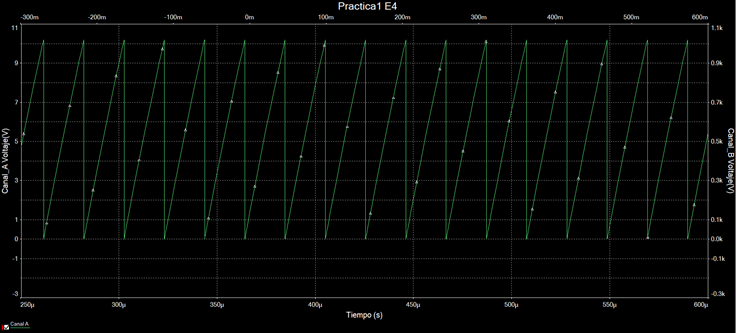
\includegraphics[width = \columnwidth]{graf_1.png}
\caption{Señal de salida, diente de sierra.}
\centering{Fuente: Elaboración propia}
\label{Gráfica}
\end{figure}

El periodo del diente de sierra, figura \ref{Gráfica}, va depender del tiempo de carga del capacitor, ya que al llegar al voltaje requerido, el SCR se activara y se descargara el capacitor por el mimso, el cual hace que inicie de nuevo el proceso de carga, y es lo que nos da una salida de diente de Sierra.\\

En la siguiente figura, figura \ref{Datos}, se puede observar el voltaje Pico de nuestra gráfica y el periodo de la misma.\\

\begin{figure}[H]
\centering
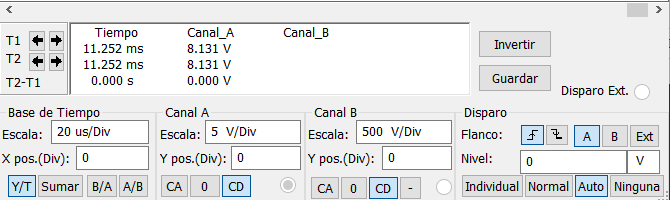
\includegraphics[width = \columnwidth]{Datos.png}
\caption{Datos del osciloscopio.}
\centering{Fuente: Elaboración propia}
\label{Datos}
\end{figure}

\subsection{Cálculos de frecuencia}

\begin{figure}[H]
\centering
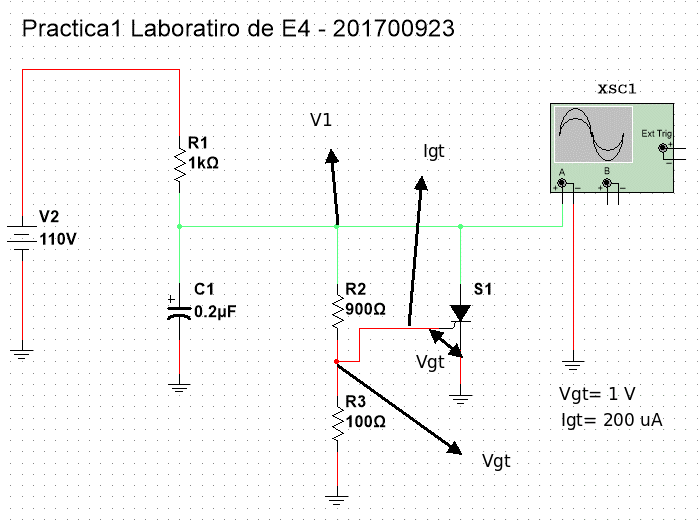
\includegraphics[width = \columnwidth]{Diagrama_calculado.png}
\caption{Identificación de nodos del circuito.}
\centering{Fuente: Elaboración propia}
\label{Datos}
\end{figure}


De la ecuación \ref{frec} podemos deducir que:\\

\begin{align*}
f_{\textup{frec}} &= \dfrac{1}{20.07 \mu s}\\
f_{\textup{frec}} &= 49825.61 Hz\\
f_{\textup{frec}} &= 49.83 kHz
\end{align*}

Sabiendo que:

\begin{align*}
I_{gt} &= 200 \mu A\\
V_{gt} &= 1 V
\end{align*}

Utilizando la ecuación $\ref{V_in}$ y $\ref{frec}$, obtenemos que:

\begin{align*}
v_{max-capacitor} &= \dfrac{900 + 100}{1 k + (900 + 100)} = 55 v\\
V_{1} &= \dfrac{1 V * (900 + 100)\Omega}{100\Omega} = 10 V
\end{align*}

%%%%%%%%%%%%%%%%%%%%%%%%%%%%%%%%%
%	Discusión de resultados		%
%%%%%%%%%%%%%%%%%%%%%%%%%%%%%%%%%

\section{Discusión de Resultados}

    %En este apartado se deben analizar los resultados obtenidos, contrastándolos con la teoría expuesta en la sección del Marco Teórico. Corresponde explicar el comportamiento de las tablas y gráficas expuestas en la sección de Resultados, tomando en cuenta el análisis estadístico apropiado.\\
    
\begin{enumerate}
	\item El voltaje pico del diente de sierra, va depende del divisor de voltaje que va al Gate, del SCR.
	
	\item El periodo del diente de sierra, va depender del tiempo de carga del capacitor, ya que al llegar al voltaje requerido, el SCR se activara y se descargara el capacitor por el mimso, el cual hace que inicie de nuevo el proceso de carga, y es lo que nos da una salida de diente de Sierra.
\end{enumerate}

%%%%%%%%%%%%%%%%%%%%%
%	Conclusiones	%
%%%%%%%%%%%%%%%%%%%%%

\section{Conclusiones}

    %Las conclusiones son interpretaciones lógicas del análisis de resultados, que deben ser consistentes con los objetivos presentados previamente.\\

\begin{enumerate}[I.]
    \item El voltaje pico del generador de diente de sierra va de la mano del divisor de voltaje que esta en el gate.
    
    \item Este generador de diente de sierra, se puede utilizar en el área de la música, para simular las ondas que podría producir un violín, cello, etc. o bien en los sintetizadores analógicos.
    
    \item Los SCR son activados principalmente por una fuente de voltaje, es decir, no es como un bjt que se activa por una corriente especifica, estos se activan principalmente por una fuente de voltaje V GT que seria el voltaje del disparador.
\end{enumerate}


%%%%%%%%%%%%%%%%%%%%%
%	Bibliografías	%
%%%%%%%%%%%%%%%%%%%%%


\begin{thebibliography}{99}
%Las fuentes de consulta se citan en forma organizada y homogénea, tanto de los libros, de los artículos y, en general, de las obras consultadas, que fueron indispensables indicar o referir en el contenido del trabajo.

\bibitem{} BOYLESTAD, ROBERT L. y NASHELSKY, LOUIS (2009) Electrónica: Teória de Circuitos y Dispositivos Electrónicos.

\bibitem{} J.A. Gualda, S. Martínez, P.M. Martínez (2001) Electrónica Industrial: Técnicas de Potencia.

\end{thebibliography}


\end{document}
